\documentclass[main.tex]{subfiles}
\begin{document}

\marginpar{Friday\\ 2019-12-13, \\ compiled \\ \today}
% \section*{Fri Dec 13 2019}

% We discuss the maximum mass of stars. 

% We were able to give meaning to the parameter \(a\): the pressure is given by 
% %
% \begin{align}
%   P(r) =
%   \frac{2 \pi}{3} G \rho_c^2 a^2 \qty(\exp(- \frac{r^2}{a^2}) - \exp(- \frac{R^2}{a^2}))
% \,,
% \end{align}
% %
% so we can see that 
% %
% \begin{align}
% a = \qty(\frac{3M}{4 \pi \rho_c \sqrt{6}})^{1/3}
% \,,
% \end{align}
% %
% and then we got an expression for the central pressure \(P_c\): the parameter multiplying it is approximately \(\num{.44}\), while more accurate models give: if \(\gamma = 5/3\) (ideal gas) we get \(\num{.48}\) whiile if \(\gamma = 4/3\) (ultrarelativistic) we get \(\num{.36}\).

% We have the relation 
% %
% \begin{align}
%   P_c = \frac{\rho _c }{\overline{m}} k_B T_c
% \,,
% \end{align}
% %
% which we use to get the last relation from last time. 

% This allows us to get some figures for main sequence (hydrogen burning) stars. 

% What is the maximum mass for Main Sequence stars? 

In the core of the star, we have both nonrelativistic and relativistic material in equilibrium: electrons and protons are nonrelativistic, while photons are relativistic.
We have discussed earlier that if most of the material in a star were relativistic it would become unstable (since, as \(\gamma \to 4/3\), the binding energy approaches 0); let us then discuss the composition of the star. 

% A star becomes unstabel when most of its material becomes ultrarelativistic: then, its total energy goes from a negative value to 0 and the adiabatic index approaches \(4/3\). 

% Suppose that the central energy is partly given by radiation and partly by matter. 
% We write
We can decompose the pressure at the core into the fractions due to nonrelativistic matter and to radiation:
%
\begin{align}
  P_c = P_m  + P_r = \beta P_c + (1 - \beta )P_c
\,,
\end{align}
%
where we define \(\beta \in (0,1)\) as the fraction of the core pressure which is due to matter: \(\beta = P_m / P_c\).

% where the terms of the two sums exactly correspond to each other, and
The two contributions can be separately expressed as:
%
\begin{align}
  \beta P_c = P_m &= \frac{\rho _c k_B T_c}{\overline{m}} \\
  (1 - \beta ) P_c = P_r &= \frac{1}{3} a T^4
\,,
\end{align}
%
where \(a\) is the radiation constant, related to the Stefan-Boltzmann constant \(\sigma \):
%
\begin{align}
  a = \frac{\pi^2   k_B^2}{15 \hbar^3 c^3}
\,.
\end{align}

We can then relate \(\beta \) to the mass of the star: in order to simplify the core temperature, we start by computing
%
\begin{align}
  \frac{\qty(\beta P_c )^{4}}{(1 - \beta ) P_c} &= \frac{\rho _c^{4}}{\overline{m}^{4}} \qty(k_B T_c)^{4} \frac{3}{a T_c^{4}}  \\
  \frac{\beta^{4}}{1 -\beta } P_c^3 &= \frac{3}{a} \qty(\frac{k_B \rho _c}{\overline{m}})^{4}
\,,
\end{align}
%
which we can invert to find an expression for the core pressure \(P_c \) in terms of \(\beta \), which we then compare to the expression we found for the core pressure as a result of the Clayton model: 
% %
% \begin{align}
%   \frac{1 - \beta }{\beta^{4}} P_c^{-3} = \frac{a}{3}
%   \qty(\frac{k_B \rho _c }{\overline{m}})^{-4}
% \,.
% \end{align}
% Inverting this we can eliminate the temperature dependence: 
%
\begin{align}
  P_c = \qty(\frac{3}{a} \frac{1 - \beta  }{\beta^{4}})^{1/3} \qty(\frac{k_B \rho _c }{\overline{m}})^{4/3}
  &= \qty(\frac{\pi }{36})^{1/3} G M^{1/3} \rho _c^{4/3} \\
  \qty(\frac{\pi }{36})^{1/3} G M^{2/3} 
  &= \qty(\frac{3}{a} \frac{(1-\beta )}{\beta^{4}})^{1/3}
  \qty(\frac{k_B}{\overline{m}})^{4/3}
\,,
\end{align}
%
the core density simplifies! 

So, if we compare stars at the same stage of fusion so that \(\overline{m}\) is constant, we have \(M \propto f(\beta ) = (1 - \beta )^{1/2} / \beta^2\).  
% so as \(\beta \) decreases, \(M\) increases. 

\(f(\beta )\) decreases as \(\beta \) increases, and it diverges to \(+ \infty \) for \(\beta \to 0\). 

Looking at the plot the other way, the heavier the star, the larger the contribution of radiation to the core pressure, which is what \(1-\beta \) quantifies.

\begin{figure}[ht]
\centering
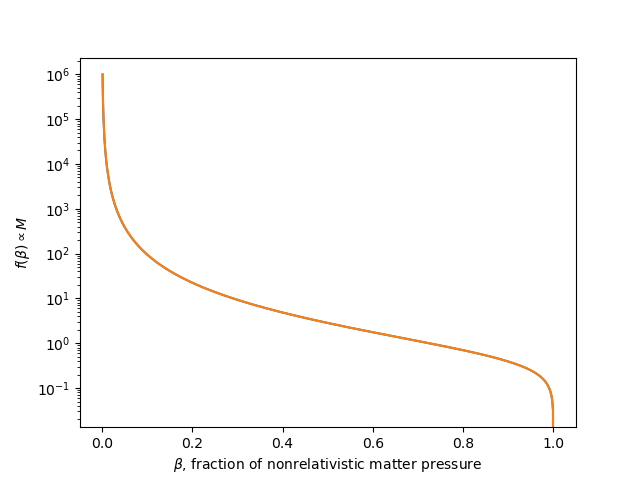
\includegraphics[width=\textwidth]{figures/beta_star_core_pressure.png}
\caption{A plot of \(f(\beta )\).}
\label{fig:beta-core-pressure}
\end{figure}
\todo[inline]{Figure made quickly, to improve by scaling it correctly, making it vector, setting the text in the right font.}

This makes sense intuitively: heavier stars reach higher temperatures and densities, so they have more radiation in the core. 

We know that for \(\beta \to 0\) the star is surely unstable, but the instability is actually reached earlier, since even before the gravitational binding energy being exactly zero large parts of the star can be flung out as stellar winds.
Proper considerations about what an appropriate critical value of \(\beta \) should be allow us to bound the stellar mass from above, at around \(50 M_{\odot}\). 

% [Plot of \(1 - \beta \) versus \(M / M_{\odot} \), showing this.]

\subsection{Degenerate electron gas}

Now we deal with the degenerate electron gas in stars. 

The distribution function is approximately given by 
%
\begin{align}
  f(p) \propto \frac{1}{\exp(\frac{\epsilon _p - \mu }{k_B T})+1}
\,,
\end{align}
%
where \(\epsilon _p = c\qty(p^2+m^2c^2)^{1/2}\). 
Then, as \(T \rightarrow 0\) we get: \(f(\epsilon _p) = 1\) if \(\epsilon _p \leq \epsilon _F\) and \(f(\epsilon _p) = 0 \) if \(\epsilon _p > \epsilon _F\); we can express this energy in terms of the momentum: 
%
\begin{align}
  \epsilon_F^2 = c^2p_F^2 + m^2 c^{4}
\,.
\end{align}

The number of electrons is given by 
%
\begin{align}
  n_e = 2 \int_{0}^{p_F} \dd{p} p^2 4 \pi \frac{1}{h^3}
  = \frac{8 \pi }{3} \qty(\frac{p_F}{h})^{3}
\,,
\end{align}
%
where we have a factor of \(2\) to account for the spin-\(1/2\) nature of the electrons. 
This means that 
%
\begin{align}
  p_F = \qty(\frac{3n}{8 \pi })^{1/3} h
\,.
\end{align}

The density is given by 
%
\begin{align}
  \rho = \frac{2}{h^3} \int_{0}^{p_F} \dd{p} p^2 4 \pi \epsilon _p
\,,
\end{align}
%
and we can consider either the nonrelativistic or the ultrarelativistic limit. In the nonrelativistic limit we find 
%
\begin{align}
  \epsilon _p = mc^2 + \frac{p^2}{2m}
\,,
\end{align}
%
so the result becomes 
%
\begin{align}
  \rho = n \qty(mc^2 + \frac{3}{10} \frac{p_F^2}{m})
\,,
\end{align}
%
and we know that for a nonrelativistic gas the pressure is given by 
%
\begin{align}
  P  = \frac{2}{3} \frac{E_k}{V}
\,,
\end{align}
%
where \(E/V\) is the kinetic energy density. 
%
\begin{align}
  P = n \frac{p_F^2}{5m}
\,,
\end{align}
%
\todo[inline]{where does this come from?}


%
\begin{align}
  P = k_{NR} n^{5/3}
\,,
\end{align}
%
where 
%
\begin{align}
  k_{NR} = \frac{h^2}{5m} \qty(\frac{3}{8 \pi })^{2/3}
\,.
\end{align}
%

In the relativistic case, on the other hand, we get \(\epsilon _p \approx cp\), and \(\rho = \frac{3}{4} n \rho _F c \). 
In this case, we also know that the pressure becomes 
%
\begin{align}
  P = \frac{1}{3} \frac{E_k}{V}
\,.
\end{align}

So we find 
%
\begin{align}
P = K_{VR} n^{4/3} 
\,,
\end{align}
%
where 
%
\begin{align}
  K_{VR} = \frac{hc}{4} \qty(\frac{3}{8 \pi })^{1/3}
\,.
\end{align}

We make a plot: on the \(x\) axis we have the number density in \(\SI{}{m^{-3}}\), on the \(y\) axis we have the temperature in \(\SI{}{K}\).

We divide the plot into: 
\begin{enumerate}
    \item Classical UR: \(P \propto n k_B T\);
    \item classical NR (like the Sun);
    \item degenerate NR: \(P = K_{NR} n^{4/3}\)
    \item degenerate UR. 
\end{enumerate}

Classical vs degenerate is marked by a line similar to \(T \sim n\), while we have NR for both \(T\) and \(n\) lower than certain critical values (since a degenerate gas can become ultrarelativistic even at low temperatures! this is the point).

We have 
%
\begin{align}
  P_c = \frac{\rho _C}{\overline{m}} k_B T_c
\,,
\end{align}
%
and 
%
\begin{align}
  k_B T_c = \qty(\frac{\pi }{36})^{1/3} G \overline{m}
  M^{2/3} \rho _c^{1/3}
\,,
\end{align}
%
and it can be (easily?) shown that 
%
\begin{align}
  \overline{m} = 2 m_H \times \frac{1}{1 + 3x_1 + 0.5 x_4}
\,,
\end{align}
%
where \(x_{1, 4}\) are the concentrations of hydrogen and helium respectively. 

To estimate the maximum achievable central temperature we do: 
%
\begin{align}
  P_c = k_{NR} n_{e}^{5/3} + n_i k_B T_c
\,,
\end{align}
%
where \(n_e = n_i  = \rho_{c} / \overline{m}_{H}\). 


%
\begin{align}
  \qty(\frac{\pi}{36})^{1/3} G M^{2/3} \rho_{c}^{4/3}
  = k_{NR} \qty(\frac{\rho_c}{m_{H}})^{5/3} + \frac{\rho_{c}}{m_H} k_B T_c
\,,
\end{align}
%
which implies 
%
\begin{align}
  k_b T_c = \qty(\frac{\pi}{36})^{1/3} G m_{H} M^{2/3} \rho_{c}^{1/3} - k_{NR} \qty(\frac{\rho_{c}}{m_H})^{2/3}
\,,
\end{align}
%
which is in the shape \(k_B T_c = A \rho_{c}^{1/3} - B \rho_{c}^{2/3}  \): we can find a maximum of this function, which comes out to be at \(\rho_{c} = (A/ 2B)^{3}\), where we have 
%
\begin{align}
  k_B T_c = \frac{A^2}{2B} = \qty(\frac{\pi }{36})^{2/3} \frac{G^2m_H^{8/3}}{4 k_{NR}} M^{4/3}
\,.
\end{align}

Now, we can set this temperature to be larger than the ignition temperature for any process we want, to see whether it will happen. 

The minimum mass is 
%
\begin{align}
  M _{\text{min}} = 
  \qty(\frac{36}{\pi })^{1/2} 
  \qty(\frac{4 k_{NR}}{G^2m_H^{8/3}})^{3/4}
  \qty(k_B T _{\text{ign}})^{3/4}
\,.
\end{align}

The potential energy between two hydrogen nuclei separated by a distance equal to their quantum wavelength is 
%
\begin{align}
E_g = - \frac{G m_H^2}{r} = - \frac{G m_H^{3}c }{\hbar}
\,,
\end{align}
%
where we inserted \(r = \hbar / m_H c\). This corresponds to an energy \(E = m_H c^2\), and we have a value 
%
\begin{align}
  \alpha_{G} = \frac{E_g}{E} =  \frac{G m_H^2}{\hbar c} \sim \SI{5.9e-39}{}
\,.
\end{align}

For electromagnetic interaction, we get 
%
\begin{align}
  \alpha_{EM} = \frac{e^2}{4 \pi \epsilon_{0} \hbar c} \approx \frac{1}{137}
\,,
\end{align}
%
which is \emph{much greater}. 

Then we find 
%
\begin{align}
  M _{\text{min}} \approx
  16 \qty(\frac{k_B T _{\text{ign}}}{m_e c^2})^{3/4}
  \alpha_{G}^{-3/2} m_H
\,.
\end{align}

If \(T _{\text{ign}} \sim \SI{1.5e6}{K}\), one tenth of the temperature of the Sun, we find 
%
\begin{align}
  M _{\text{min}} \sim \num{.03} \alpha_{G}^{-3/2} m_H
\,,
\end{align}
%
while for the maximum mass, from before with \(\beta = \num{.5}\) and \(\overline{m} = \num{.61} m_H\) we get 
%
\begin{align}
  M _{\text{max}} \approx 56 \alpha_{G}^{-3/2} m_H
\,,
\end{align}
%
so this hints to the fact that \(m_{*} = \alpha_{G}^{-3/2} m_H \) is an important characteristic mass. This is around \(\num{1.85} M_{\odot}\). 

This corresponds to a number of particles: 
%
\begin{align}
  N_{*} = \frac{m_{*}}{m_H} \approx \num{2e52}
\,.
\end{align}

Suppose the core of a star is held together by the pressure of degenerate electrons: we discuss \emph{white dwarves}.
We define 
%
\begin{align}
  n_e = Y_{e} \frac{\rho_{c}}{m_H}
\,,
\end{align}
%
where \(Y_e = (1 + x_1) /2\).
The pressure is 
%
\begin{align}
  P = k_{NR} n_e^{5/3} = k_{NR} \qty(\frac{Y_e \rho_{c}}{m_H})^{5/3}
\,,
\end{align}
%
which must compared to 
%
\begin{align}
  P_c = \qty(\frac{\pi }{36})^{1/3} G M^{2/3} \rho_{c}^{4/3}
\,,
\end{align}
%
and we assume that \(P = P_c\): then we get 
%
\begin{align}
  \rho_{c} \approx \frac{\num{3.1}}{Y_e^{5}} \frac{M}{m_{*}} \frac{m_H}{(h / m_e c^2)^{3}}
\,.
\end{align}

\todo[inline]{
  Missing square on the \(M / m_*\)?
}

The pressure is 
%
\begin{align}
P = k_{UR} n_e^{4/3} 
= k_{UR}\qty(\frac{Y_e \rho_{c}}{m_H})^{4/3}
\,,
\end{align}
%
so we get 
%
\begin{align}
  k_{UR} \qty(\frac{Y_e \rho_{c}}{m_H})^{4/3} \approx 
  \qty(\frac{\pi }{36})^{1/3} G M^{2/3} \rho_{c}^{4/3}
\,,
\end{align}
%
so we can see that in this limit the expression becomes independent of \(\rho_{c}\). This will give us a limit mass: the Chandrasekhar mass.  
%
\begin{align}
  M_{CH} = 
  \qty(\frac{36}{\pi } )^{1/2} \qty(\frac{Y_e}{m_H})^2
  \qty(\frac{k_{UR}}{G})^{3/2} \approx 2.3 Y_e^2 m_{*} \approx 4.3 Y_e^2 M_{\odot} \approx 1.4 M_{\odot}
\,.
\end{align}

This is the maximum mass of a white dwarf to remain stable, held together by the degeneracy pressure of electrons. 
Above this, it becomes a neutron star.

\end{document}